\chapter{Studi Kasus dan Pembahasan}

\begin{mybox}{Anggota kelompok}
	\begin{enumerate}
		\itemsep0em
		\item ENGELBERTUS RANDE (NIM 25/573149/PPA/07211)
		\item GILBERT FANDILIAM MOOY (NIM 25/574767/PPA/07259)
		\item Sinta Siti Nuriah (NIM 25/575177/PPA/07274)
		\item Vicky Mahfudy (NIM 25/573019/PPA/07207)
	\end{enumerate}
\end{mybox}

\section{Skema Data Base \& Data Warehouse}

Skema pada sistem *Data Warehouse* ini menggunakan dataset \textit{ClassicModels}. Data bersumber dari *dump file* MySQL yang berisi rekam jejak sistem OLTP dan diubah ke dalam bentuk OLAP menggunakan DuckDB. Tabel yang dihasilkan meliputi tabel dimensi dan fakta seperti rincian pelanggan, produk, transaksi pesanan, dan pembayaran.

\begin{table}[H]
	\centering
	\caption{Ringkasan Baris Tabel pada DuckDB}
	\begin{tabularx}{0.7\textwidth}{@{} X r @{}}
		\toprule
		\textbf{Nama Tabel} & \textbf{Jumlah Baris (Rows)} \\ \midrule
		customers & 122 \\
		employees & 23 \\
		offices & 7 \\
		orderdetails & 2.996 \\
		orders & 326 \\
		payments & 273 \\
		productlines & 7 \\
		products & 110 \\ \bottomrule
	\end{tabularx}
\end{table}

\section{Skenario dan Penyelesaian}

Berikut adalah langkah-langkah detail implementasi yang dieksekusi secara berurutan melalui lingkungan komputasi \textit{Jupyter Notebook} di Google Colab.

\subsection{Background and Setup}
Langkah awal ini berfokus pada persiapan lingkungan kerja dengan menginstal alat pemodelan data (dbt) dan sistem basis data (DuckDB), serta memastikan semuanya berada pada versi yang sesuai.

\begin{lstlisting}[language=bash, numbers=left, caption={Instalasi Library}]
	!pip install dbt-core dbt-duckdb duckdb pandas
\end{lstlisting}

\begin{lstlisting}[language=bash, numbers=left, caption={Output: Log Instalasi (Singkat)}]
	Collecting dbt-core
	Downloading dbt_core-1.11.8-py3-none-any.whl.metadata (4.4 kB)
	Collecting dbt-duckdb
	Downloading dbt_duckdb-1.10.1-py3-none-any.whl.metadata (38 kB)
	Requirement already satisfied: duckdb in /usr/local/lib/python3.12/dist-packages (1.3.2)
	Requirement already satisfied: pandas in /usr/local/lib/python3.12/dist-packages (2.2.2)
	...
	Successfully installed agate-1.9.1 colorama-0.4.6 daff-1.4.2 dbt-adapters-1.22.10 dbt-common-1.38.0 dbt-core-1.11.8 dbt-duckdb-1.10.1 ...
\end{lstlisting}

\begin{lstlisting}[language=bash, numbers=left, caption={Verifikasi Versi dbt}]
	!dbt --version
\end{lstlisting}

\begin{lstlisting}[language=bash, numbers=left, caption={Output: Versi dbt}]
	Core:
	- installed: 1.11.8
	- latest:    1.11.8 - Up to date!
	
	Plugins:
	- duckdb: 1.10.1 - Up to date!
\end{lstlisting}

\begin{lstlisting}[language=Python, numbers=left, caption={Verifikasi Versi DuckDB}]
	!python -c "import duckdb; print(duckdb.__version__)"
	# Output:
	# 1.3.2
\end{lstlisting}

\begin{lstlisting}[language=Python, numbers=left, caption={Koneksi ke Google Drive}]
	from google.colab import drive
	drive.mount('/content/drive')
	# Output: Drive already mounted at /content/drive...
\end{lstlisting}

\subsection{Convert MySQL to DuckDB}
Data asli berada dalam format file *dump* SQL yang memiliki sintaks spesifik MySQL. Proses ini akan membersihkan sintaks tersebut (misalnya, menghapus parameter \textit{ENGINE}, mengubah *backticks*, dan merapikan klausa \textit{FOREIGN KEY}) agar kompatibel untuk dieksekusi di DuckDB.
\clearpage
\begin{lstlisting}[language=Python, numbers=left, caption={Konfigurasi Path}]
	import os
	# --- PENGATURAN PATH GOOGLE DRIVE ---
	DRIVE_BASE = "/content/drive/MyDrive/Term 1/Data Warehouse/Tugas DBT"
	INPUT_FILE = DRIVE_BASE+"/mysqlsampledatabase.sql"
	DUCKDB_FILE = DRIVE_BASE+"/classicmodels.duckdb"
	OUTPUT_FILE = os.path.join(DUCKDB_FILE)
\end{lstlisting}

\begin{lstlisting}[language=Python, numbers=left, caption={Script ETL: Pembersihan dan Ingesti SQL}]
	import re
	import duckdb
	from google.colab import drive
	
	# 1. Mount Google Drive
	drive.mount('/content/drive')
	
	def convert_mysql_to_duckdb(input_sql_path, output_duckdb_path):
	if not os.path.exists(input_sql_path):
	print(f"File {input_sql_path} tidak ditemukan!")
	return
	
	print(f"Membaca file: {input_sql_path}...")
	with open(input_sql_path, 'r', encoding='latin-1') as f:
	sql_content = f.read()
	
	print("Membersihkan sintaks MySQL...")
	
	# 1. Hapus komentar dan metadata MySQL level database
	sql_content = re.sub(r'/\*.*?\*/', '', sql_content, flags=re.DOTALL)
	sql_content = re.sub(r'--.*?\n', '\n', sql_content)
	sql_content = re.sub(r'(?i)CREATE DATABASE.*?;', '', sql_content)
	sql_content = re.sub(r'(?i)USE\s+\w+;', '', sql_content)
	
	# 2. FIX KOLOM & TABEL (Penting untuk addressLine1, dsb)
	sql_content = re.sub(r'`(\w+)`', r'"\1"', sql_content)
	
	# 3. Sesuaikan tipe data
	sql_content = re.sub(r'(?i)\bmediumtext\b', 'TEXT', sql_content)
	sql_content = re.sub(r'(?i)\bmediumblob\b', 'BLOB', sql_content)
	sql_content = re.sub(r'(?i)\bsmallint\(\d+\)', 'SMALLINT', sql_content)
	sql_content = re.sub(r'(?i)\bint\(\d+\)', 'INTEGER', sql_content)
	
	# 4. Perbaiki Escape Characters & Tanggal
	sql_content = sql_content.replace(r"\'", "''")
	sql_content = sql_content.replace("'0000-00-00'", "NULL")
	
	# 5. Hapus engine-specific MySQL
	sql_content = re.sub(r'(?i)ENGINE=\w+', '', sql_content)
	sql_content = re.sub(r'(?i)DEFAULT CHARSET=\w+', '', sql_content)
	sql_content = re.sub(r'(?i)COLLATE=\w+', '', sql_content)
	
	# 6. Hapus baris FOREIGN KEY
	lines = sql_content.split('\n')
	cleaned_lines = []
	for line in lines:
	if 'FOREIGN KEY' in line.upper(): continue
	if 'KEY ' in line.upper() and 'PRIMARY' not in line.upper(): continue
	cleaned_lines.append(line)
	
	sql_content = '\n'.join(cleaned_lines)
	
	# 7. Bersihkan koma gantung (dangling comma)
	sql_content = re.sub(r',\s*\)', '\n)', sql_content)
	
	# --- PROSES EKSEKUSI ---
	if os.path.exists(output_duckdb_path):
	os.remove(output_duckdb_path)
	
	print(f"Mengeksekusi ke DuckDB di: {output_duckdb_path}")
	conn = duckdb.connect(output_duckdb_path)
	statements = re.split(r';\s*\n', sql_content)
	
	success_count = 0
	error_count = 0
	
	for stmt in statements:
	clean_stmt = stmt.strip()
	if clean_stmt:
	try:
	conn.execute(clean_stmt + ";")
	success_count += 1
	except Exception as e:
	if "DROP" not in clean_stmt.upper():
	print(f"Warning pada: {clean_stmt[:50]}... \n Detail: {e}")
	error_count += 1
	
	print(f"\nSelesai! Berhasil: {success_count}, Gagal: {error_count}")
	
	# Tampilkan Ringkasan Tabel
	print("\n" + "="*40)
	print(f"{'TABEL':<20} | {'JUMLAH BARIS':>10}")
	print("-" * 40)
	try:
	tables = conn.execute("SHOW TABLES").fetchall()
	for (t,) in tables:
	count = conn.execute(f'SELECT COUNT(*) FROM "{t}"').fetchone()[0]
	print(f"{t:<20} | {count:>10}")
	except:
	pass
	conn.close()
	
	if __name__ == "__main__":
	if not os.path.exists(DRIVE_BASE):
	os.makedirs(DRIVE_BASE)
	convert_mysql_to_duckdb(INPUT_FILE, OUTPUT_FILE)
\end{lstlisting}

\begin{lstlisting}[language=bash, numbers=left, caption={Output: Hasil Eksekusi Pembuatan DuckDB}]
	Membaca file: /content/drive/MyDrive/Term 1/Data Warehouse/Tugas DBT/mysqlsampledatabase.sql...
	Membersihkan sintaks MySQL...
	Mengeksekusi ke DuckDB di: /content/drive/MyDrive/Term 1/Data Warehouse/Tugas DBT/classicmodels.duckdb
	
	Selesai! Berhasil: 24, Gagal: 0
	
	========================================
	TABEL                | JUMLAH BARIS
	----------------------------------------
	customers            |        122
	employees            |         23
	offices              |          7
	orderdetails         |       2996
	orders               |        326
	payments             |        273
	productlines         |          7
	products             |        110
\end{lstlisting}

Selanjutnya, dilakukan verifikasi skema pada \textit{schema main} dari objek \textit{database} DuckDB yang telah dibuat.

\begin{lstlisting}[language=Python, numbers=left, caption={Verifikasi Skema pada Data Warehouse}]
	## Pengecekan sampel dengan mengambil 3 baris
	
	# Buka koneksi ke file database yang sudah dikonversi
	con = duckdb.connect(DUCKDB_FILE)
	
	# -- 1. List all tables --------------------------------------------------------
	print("=" * 50)
	print("Source tables in 'main' schema")
	print("=" * 50)
	tables = con.execute("""
	SELECT table_name
	FROM   information_schema.tables
	WHERE  table_schema = 'main'
	ORDER  BY table_name
	""").fetchall()
	
	for (t,) in tables:
	print(f"  {t}")
	
	print(f"\nTotal: {len(tables)} tables")
	expected = {'customers', 'employees', 'offices', 'orderdetails',
		'orders', 'payments', 'productlines', 'products'}
	found = {t for (t,) in tables}
	missing = expected - found
	if missing:
	print(f"\n[WARN] Missing expected tables: {missing}")
	else:
	print("[OK] All 8 expected tables found.")
	
	# -- 2. Row counts per table ---------------------------------------------------
	print("\n" + "=" * 50)
	print("Row counts")
	print("=" * 50)
	for (t,) in tables:
	count = con.execute(f"SELECT COUNT(*) FROM {t}").fetchone()[0]
	print(f"  {t:<20} {count:>6} rows")
	
	# -- 3. Sample: first 3 rows of each table ------------------------------------
	print("\n" + "=" * 50)
	print("Sample rows (first 3 per table)")
	print("=" * 50)
	for (t,) in tables:
	print(f"\n-- {t} --")
	df = con.execute(f"SELECT * FROM {t} LIMIT 3").df()
	print(df.to_string(index=False))
	
	con.close()
\end{lstlisting}

\begin{lstlisting}[language=bash, numbers=left, caption={Output: Pengecekan sampel baris}]
	==================================================
	Source tables in 'main' schema
	==================================================
	customers
	employees
	offices
	orderdetails
	orders
	payments
	productlines
	products
	
	Total: 8 tables
	[OK] All 8 expected tables found.
	
	==================================================
	Row counts
	==================================================
	customers               122 rows
	employees                23 rows
	offices                   7 rows
	orderdetails           2996 rows
	orders                  326 rows
	payments                273 rows
	productlines              7 rows
	products                110 rows
	
	==================================================
	Sample rows (first 3 per table)
	==================================================
	
	-- customers --
	customerNumber               customerName contactLastName contactFirstName        phone      addressLine1 addressLine2      city    state postalCode   country  salesRepEmployeeNumber  creditLimit
	103          Atelier graphique         Schmitt          Carine    40.32.2555    54, rue Royale         None    Nantes     None      44000    France                    1370      21000.0
	112         Signal Gift Stores            King             Jean   7025551838   8489 Strong St.         None Las Vegas       NV      83030       USA                    1166      71800.0
	114 Australian Collectors, Co.        Ferguson            Peter 03 9520 4555 636 St Kilda Road      Level 3 Melbourne Victoria       3004 Australia                    1611     117300.0
	
	-- employees --
	employeeNumber  lastName firstName extension                          email officeCode  reportsTo     jobTitle
	1002    Murphy     Diane     x5800   dmurphy@classicmodelcars.com          1       <NA>    President
	1056 Patterson      Mary     x4611 mpatterso@classicmodelcars.com          1       1002     VP Sales
	1076  Firrelli      Jeff     x9273 jfirrelli@classicmodelcars.com          1       1002 VP Marketing
	
	-- offices --
	officeCode          city           phone         addressLine1 addressLine2 state country postalCode territory
	1 San Francisco +1 650 219 4782    100 Market Street    Suite 300    CA     USA      94080        NA
	2        Boston +1 215 837 0825     1550 Court Place    Suite 102    MA     USA      02107        NA
	3           NYC +1 212 555 3000 523 East 53rd Street      apt. 5A    NY     USA      10022        NA
	
	-- orderdetails --
	orderNumber productCode  quantityOrdered  priceEach  orderLineNumber
	10100    S18_1749               30     136.00                3
	10100    S18_2248               50      55.09                2
	10100    S18_4409               22      75.46                4
	
	-- orders --
	orderNumber  orderDate requiredDate shippedDate  status               comments  customerNumber
	10100 2003-01-06   2003-01-13  2003-01-10 Shipped                   None             363
	10101 2003-01-09   2003-01-18  2003-01-11 Shipped Check on availability.             128
	10102 2003-01-10   2003-01-18  2003-01-14 Shipped                   None             181
	
	-- payments --
	customerNumber checkNumber paymentDate   amount
	103    HQ336336  2004-10-19  6066.78
	103    JM555205  2003-06-05 14571.44
	103    OM314933  2004-12-18  1676.14
	
	-- productlines --
	productLine    textDescription                         htmlDescription image
	Classic Cars   Attention car enthusiasts...            None            <NA>
	Motorcycles    State-of-the-art replicas...            None            <NA>
	Planes         Diecast airplane replicas...            None            <NA>
	
	-- products --
	productCode productName                       productLine  stock buyPrice MSRP
	S10_1678    1969 Harley Davidson Chopper      Motorcycles  7933   48.81  95.70
	S10_1949    1952 Alpine Renault 1300          Classic Cars 7305   98.58 214.30
	S10_2016    1996 Moto Guzzi 1100i             Motorcycles  6625   68.99 118.94
\end{lstlisting}

\subsection{Working with dbt \& Profiles Configuration}
Untuk mengeksekusi model analitik, proyek dbt diinisialisasi dan diatur profil koneksinya agar merujuk ke file \textit{database} DuckDB (\texttt{classicmodels.duckdb}).

\begin{lstlisting}[language=Python, numbers=left, caption={Konfigurasi profiles.yml}]
	profiles_yaml = f"""
	classicmodels:
	target: dev
	outputs:
	dev:
	type: duckdb
	path: {DUCKDB_FILE}
	threads: 1
	"""
	with open("profiles.yml", "w") as f:
	f.write(profiles_yaml)
\end{lstlisting}

\section{Part 3: Building the Data Marts with dbt}

Bagian ini merupakan inti dari seluruh proses pemodelan data menggunakan dbt (\textit{data build tool}). Arsitektur yang dibangun mengikuti pola tiga lapisan (\textit{three-tier architecture}): \textit{Staging Layer} untuk pembersihan, \textit{Dimension Layer} untuk data master, dan \textit{Marts Layer} untuk tabel fakta.

\subsection{Step 1: Verify the Source Data}
Sebelum melakukan transformasi, dilakukan verifikasi integritas data pada \textit{Source Database}. Langkah ini memastikan bahwa tabel mentah telah terbaca dengan benar.

\begin{lstlisting}[language=Python, caption=Verifikasi Data Sumber]
# Preview relasi antara orders dan customers
results = conn.execute("""
    SELECT o.orderNumber, o.status, c.customerName
    FROM orders o
    JOIN customers c USING (customerNumber)
    LIMIT 3;
""").df()
print(results)
\end{lstlisting}

\textbf{Contoh Output:}
\begin{verbatim}
   orderNumber    status             customerName
0        10100   Shipped      Online Diecast Creations
1        10101   Shipped          Blauer See Auto, Co.
2        10102   Shipped             Vitachrome Inc.
\end{verbatim}

\subsection{Step 2: Build the Staging Layer}
\textit{Staging layer} melakukan standarisasi nama kolom. Misalnya, mengubah \texttt{customerNumber} menjadi \texttt{customer\_id} agar lebih konsisten (snake\_case).

\begin{lstlisting}[language=SQL, caption=stg\_products.sql]
select
    productCode as product_code,
    productName as product_name,
    quantityInStock as qty_stock,
    buyPrice as buy_price
from {{ source('main', 'products') }}
\end{lstlisting}

\subsection{Step 3: Dimensional Modeling (Business Processes)}

Berikut adalah implementasi lima proses bisnis utama:
\begin{enumerate}
    \item Business Process 1: Sales Order Lines
    \item Business Process 2: Customer Payments
    \item Business Process 3: Sales Rep Performance
    \item Business Process 4: Order Fulfillment \& Logistics
    \item Business Process 5: Inventory Valuation \& Product
\end{enumerate}
Berikut implementasi yang dapat dilakukan untuk Dimensional modelingnya.
\subsubsection{Business Process 1: Sales Order Lines}
Tabel \texttt{fct\_order\_lines} menganalisis pendapatan dan margin keuntungan
pada tingkat granularitas item pesanan, di mana satu baris merepresentasikan
satu produk dalam satu pesanan (\textit{grain}: 1 item $\times$ 1 order).
Model ini menggabungkan lima tabel staging: \texttt{stg\_orderdetails},
\texttt{stg\_orders}, \texttt{stg\_products}, \texttt{stg\_customers}, dan
\texttt{stg\_employees}.

Tiga \textit{measures} dihitung langsung pada level baris:
\textit{revenue} (\texttt{quantity\_ordered $\times$ price\_each}),
\textit{total\_cost} (\texttt{quantity\_ordered $\times$ buy\_price}), dan
\textit{gross\_profit} selisih keduanya. Output agregasi utama adalah
\textbf{Total Revenue} sebagai KPI utama Dashboard Penjualan.

\begin{lstlisting}[
  language=SQL,
  caption={models/marts/fct\_order\_lines.sql},
  label={lst:fct-order-lines},
  basicstyle=\ttfamily\footnotesize,
  keywordstyle=\color{blue!70!black}\bfseries,
  commentstyle=\color{gray}\itshape,
  stringstyle=\color{orange!80!black},
  showstringspaces=false,
  breaklines=true,
  frame=single,
  numbers=left,
  numberstyle=\tiny\color{gray},
  numbersep=8pt,
  xleftmargin=15pt
]
with order_details as (
    select * from {{ ref('stg_orderdetails') }}
),
orders     as ( select * from {{ ref('stg_orders') }} ),
products   as ( select * from {{ ref('stg_products') }} ),
customers  as ( select * from {{ ref('stg_customers') }} ),
employees  as ( select * from {{ ref('stg_employees') }} )

select
    -- Keys
    md5(od.order_id || '-' || od.product_code) as order_line_key,
    od.order_id,
    od.product_code,
    o.customer_id,
    o.order_date,
    c.sales_rep_employee_id                    as employee_id,
    e.office_code,

    -- Measures
    od.quantity_ordered,
    od.price_each,
    (od.quantity_ordered * od.price_each)      as revenue,
    p.buy_price,
    (od.quantity_ordered * p.buy_price)        as total_cost,
    ((od.quantity_ordered * od.price_each)
     - (od.quantity_ordered * p.buy_price))    as gross_profit

from order_details od
join orders    o on od.order_id     = o.order_id
join products  p on od.product_code = p.product_code
join customers c on o.customer_id   = c.customer_id
join employees e on c.sales_rep_employee_id = e.employee_id
\end{lstlisting}

Fungsi \texttt{md5()} menghasilkan \textit{surrogate key} yang unik dan
deterministik dari kombinasi \texttt{order\_id} dan \texttt{product\_code}.
Penggunaan \texttt{\{\{ ref() \}\}} membangun dependensi antar-model secara
otomatis sehingga dbt dapat menentukan urutan eksekusi yang benar dan
menampilkan DAG \textit{lineage} pada \texttt{dbt docs}.


\subsubsection{Business Process 2: Customer Payments}

\textbf{Skenario Bisnis:} 
Proses bisnis kedua berfokus pada pemantauan arus kas (\textit{cash flow}). Manajemen perlu menghubungkan data pembayaran dengan profil pelanggan (\texttt{customer\_id}) untuk mengukur likuiditas perusahaan dan perilaku pembayaran pelanggan.

\textbf{Grain:} 
Satu baris per transaksi pembayaran (\textit{one row per payment transaction}).

\textbf{Penjelasan Logika dbt:}
\begin{itemize}
    \item \textbf{dim\_date}: Dibuat secara dinamis dengan menggabungkan (\textit{union}) tanggal unik dari tabel \texttt{orders} dan \texttt{payments} untuk memastikan dimensi waktu mencakup seluruh rentang aktivitas bisnis.
    \item \textbf{fct\_payments}: Menggunakan \textit{Surrogate Key} berupa \texttt{md5} yang menggabungkan \texttt{customer\_id} dan \texttt{check\_number} untuk menjamin keunikan tiap baris fakta.
\end{itemize}

\begin{lstlisting}[language=Python, caption=Skrip Python untuk Penyiapan Model Customer Payments]
def setup_dbt_content():
    # Menyiapkan direktori model
    folders = ["models/dimensions", "models/marts"]
    for folder in folders:
        os.makedirs(os.path.join(PROJECT_BASE, folder), exist_ok=True)

    # Definisi file Marts dan Dimensions
    mart_files_2 = {
        "models/dimensions/dim_date.sql": """
            with all_dates as (
                select order_date as date_day from {{ ref('stg_orders') }}
                union
                select payment_date as date_day from {{ ref('stg_payments') }}
            )
            select
                distinct(date_day) as date_day,
                year(date_day)     as year,
                month(date_day)    as month,
                dayname(date_day)  as day_name
            from all_dates """,

        "models/marts/fct_payments.sql": """
            select
                md5(customer_id || '-' || check_number) as payment_key,
                customer_id,
                payment_date,
                check_number,
                amount
            from {{ ref('stg_payments') }} """
    }

    # Proses penulisan file SQL ke dalam sistem
    for rel_path, content in mart_files_2.items():
        full_path = os.path.join(PROJECT_BASE, rel_path)
        with open(full_path, "w") as f:
            f.write(content.strip())
    
	    print("[OK] data marts siap!")

if __name__ == "__main__":
    setup_dbt_content()
\end{lstlisting}

\textbf{Output pada Notebook (IPYNB):}
\begin{verbatim}
[INFO] Menyiapkan model di: /content/drive/MyDrive/.../classicmodels_dw
[OK] data marts siap!
\end{verbatim}

\subsubsection{Business Process 3: Sales Rep Performance}
Mengukur kinerja tenaga penjual secara bulanan. 
\textbf{Output:} Digunakan untuk menghitung bonus tahunan karyawan.
Tabel \texttt{fct\_sales\_performance} mengukur kinerja tenaga penjual secara
bulanan dengan \textit{grain}: 1 sales rep $\times$ 1 bulan. Berbeda dengan
\texttt{fct\_order\_lines} yang beroperasi pada level transaksi atomik, model
ini merupakan \textit{periodic snapshot} yang mengagregasi seluruh aktivitas
penjualan per karyawan dalam satu periode bulan. Output utamanya digunakan
sebagai dasar perhitungan \textbf{bonus tahunan karyawan}.
 
Model ini tidak membaca tabel sumber secara langsung, melainkan membangun
di atas \texttt{fct\_order\_lines} menggunakan \texttt{\{\{ ref() \}\}},
sehingga membentuk lapisan mart-on-mart yang menjaga konsistensi definisi
metrik di seluruh pipeline.
 
\begin{lstlisting}[
  language=SQL,
  caption={models/marts/fct\_sales\_performance.sql},
  label={lst:fct-sales-perf},
  basicstyle=\ttfamily\footnotesize,
  keywordstyle=\color{blue!70!black}\bfseries,
  commentstyle=\color{gray}\itshape,
  stringstyle=\color{orange!80!black},
  showstringspaces=false,
  breaklines=true,
  frame=single,
  numbers=left,
  numberstyle=\tiny\color{gray},
  numbersep=8pt,
  xleftmargin=15pt
]
with order_lines as (
    select * from {{ ref('fct_order_lines') }}
),
 
performance_snapshot as (
    select
        employee_id,
        office_code,
        -- Hari pertama setiap bulan sebagai kunci periode
        date_trunc('month', order_date)  as month_date,
 
        -- Aggregated Measures
        count(distinct order_id)         as order_count,
        count(distinct customer_id)      as unique_customers,
        sum(quantity_ordered)            as total_units_sold,
        sum(revenue)                     as total_revenue,
        sum(gross_profit)                as total_gross_profit,
        avg(revenue)                     as avg_order_line_revenue
 
    from order_lines
    -- Hanya transaksi yang memiliki sales rep terdaftar
    where employee_id is not null
    group by
        employee_id,
        office_code,
        date_trunc('month', order_date)
)
 
select
    -- Surrogate Key
    md5(cast(employee_id as varchar)
        || '-' || cast(month_date as varchar)) as performance_key,
 
    -- Dimensions
    employee_id,
    office_code,
    month_date,
 
    -- Measures
    order_count,
    unique_customers,
    total_units_sold,
    total_revenue,
    total_gross_profit,
    avg_order_line_revenue
 
from performance_snapshot
\end{lstlisting}
 
Terdapat beberapa keputusan teknis penting pada model ini. Pertama,
\texttt{date\_trunc('month', order\_date)} menormalisasi setiap tanggal
transaksi menjadi hari pertama bulan tersebut, sehingga seluruh aktivitas
dalam satu bulan dapat dikelompokkan di bawah satu kunci periode yang
konsisten. Kedua, filter \texttt{WHERE employee\_id IS NOT NULL} memastikan
hanya transaksi yang dapat diatribusikan kepada sales rep tertentu yang
masuk ke dalam perhitungan, menghindari distorsi pada agregasi kinerja.
Ketiga, surrogate key \texttt{performance\_key} dibuat dari kombinasi
\texttt{employee\_id} dan \texttt{month\_date}, menjamin keunikan setiap
baris snapshot bulanan.
 
Enam \textit{measures} yang dihasilkan mencakup aspek volume
(\texttt{order\_count}, \texttt{total\_units\_sold}), jangkauan pelanggan
(\texttt{unique\_customers}), serta finansial (\texttt{total\_revenue},
\texttt{total\_gross\_profit}, \texttt{avg\_order\_line\_revenue}) yang
secara bersama-sama membentuk profil kinerja komprehensif per karyawan
per bulan sebagai input kalkulasi bonus tahunan.
\subsubsection{Business Process 4: Order Fulfillment \& Logistics}
\subsection{Skenario Bisnis}
Manajer Logistik dan Operasional perlu menganalisis efisiensi proses pemenuhan pesanan (\textit{order fulfillment}). Fokus utama adalah melacak berapa lama waktu yang dibutuhkan untuk mengirim pesanan, mengidentifikasi hambatan (\textit{bottlenecks}) atau keterlambatan, serta memantau performa pengiriman (\textit{on-time vs. delayed}) di berbagai wilayah pelanggan dan periode waktu.

\subsection{Perancangan Tabel Fakta}
Tabel fakta ini menggunakan pendekatan \textbf{Accumulating Snapshot Fact Table}. Berbeda dengan tabel fakta transaksi, baris dalam tabel ini diperbarui secara logis saat pesanan bergerak melalui siklus hidupnya (dari \textit{ordered} $\rightarrow$ \textit{required} $\rightarrow$ \textit{shipped}).

\begin{itemize}
    \item \textbf{Grain:} Satu baris per pesanan — mewakili siklus hidup lengkap dari satu pesanan penjualan tunggal.
    \item \textbf{Fact Table:} \texttt{fct\_order\_fulfillment}
\end{itemize}

\subsection{Dimensi dan Metrik}
\subsubsection{Dimensi}
\begin{itemize}
    \item \textbf{dim\_customer:} Informasi siapa yang memesan dan ke mana pesanan dikirim (kota/negara).
    \item \textbf{Role-Playing Date Dimensions:} Kita menggunakan tabel \texttt{dim\_date} yang sama, namun dihubungkan tiga kali untuk kejadian yang berbeda:
    \begin{itemize}
        \item \textit{dim\_order\_date}: Saat pesanan dibuat.
        \item \textit{dim\_required\_date}: Batas waktu pengiriman.
        \item \textit{dim\_shipped\_date}: Saat pesanan benar-benar keluar dari gudang.
    \end{itemize}
    \item \textbf{dim\_status:} \textit{Degenerate dimension} yang mewakili status pesanan (Shipped, In Process, Cancelled, On Hold).
\end{itemize}

\subsubsection{Measures (Metrik)}
\begin{itemize}
    \item \textbf{days\_to\_ship:} Jumlah hari antara \texttt{orderDate} dan \texttt{shippedDate}.
    \item \textbf{days\_delayed:} Jumlah hari keterlambatan terhadap \texttt{requiredDate}.
    \item \textbf{is\_delayed\_flag:} Penanda (1 atau 0) jika pesanan dikirim melewati batas waktu.
    \item \textbf{total\_items\_in\_order:} Jumlah produk dalam pesanan tersebut.
\end{itemize}

\subsection{Arsitektur Star Schema}
Gambar berikut mengilustrasikan arsitektur \textit{star schema} untuk proses \textit{Order Fulfillment \& Logistics}.

\begin{figure}[H]
    \centering
    \resizebox{\textwidth}{!}{%
    \begin{tikzpicture}[
        node distance=1cm,
        fact/.style={rectangle, draw, fill=purple!15, text width=3.5cm, align=left, rounded corners, font=\small},
        dim/.style={rectangle, draw, fill=teal!15, text width=3cm, align=left, rounded corners, font=\small},
        dimdate/.style={rectangle, draw, fill=blue!12, text width=3cm, align=left, rounded corners, font=\small},
        dimstatus/.style={rectangle, draw, fill=orange!15, text width=3.8cm, align=left, rounded corners, font=\small},
    ]

    %% Fact Table (center)
    \node[fact] (fact) {
        \textbf{fct\_order\_fulfillment} \\
        \rule{\linewidth}{0.4pt} \\
        \underline{customer\_key (FK)} \\
        \underline{order\_date\_key (FK)} \\
        \underline{required\_date\_key (FK)} \\
        \underline{shipped\_date\_key (FK)} \\
        status \textit{(degenerate)} \\
        \rule{\linewidth}{0.4pt} \\
        days\_to\_ship \\
        days\_delayed \\
        is\_delayed\_flag \\
        total\_items\_in\_order
    };

    %% dim_customer (left)
    \node[dim, left=3cm of fact] (dimcust) {
        \textbf{dim\_customer} \\
        \rule{\linewidth}{0.4pt} \\
        \underline{customer\_key (PK)} \\
        customer\_name \\
        city / country \\
        contact\_info
    };

    %% dim_date (top) — shared, role-playing 3×
    \node[dimdate, above=2.5cm of fact] (dimdate) {
        \textbf{dim\_date} \textit{(role-playing)} \\
        \rule{\linewidth}{0.4pt} \\
        \underline{date\_key (PK)} \\
        full\_date \\
        day / month / year \\
        day\_of\_week / quarter
    };

    %% dim_status (right) — degenerate
    \node[dimstatus, right=3cm of fact] (dimstat) {
        \textbf{dim\_status} \\
        \textit{(degenerate dimension)} \\
        \rule{\linewidth}{0.4pt} \\
        Shipped \\
        In Process \\
        Cancelled \\
        On Hold
    };

    %% Arrows
    \draw[->] (dimcust) -- node[above, font=\tiny]{1 : N} (fact);
    \draw[->] (dimdate) -- node[pos=0.1, right, font=\tiny]{order\_date}
              ([xshift=-0.5cm]fact.north);
    \draw[->, dashed] (dimdate) -- node[pos=0.5, right, font=\tiny]{required\_date}
              (fact.north);
    \draw[->, dotted] (dimdate) -- node[pos=0.7, right, font=\tiny]{shipped\_date}
              ([xshift=0.5cm]fact.north);
    \draw[->, dashed] (fact) -- node[above, font=\tiny]{degenerate} (dimstat);

    \end{tikzpicture}%
    }
    \caption{Star Schema --- \texttt{fct\_order\_fulfillment} (Accumulating Snapshot)}
    \label{fig:star-schema-fulfillment}
\end{figure}

\subsection{Implementasi dbt (Data Transformation)}
Langkah ini melibatkan pembuatan model SQL di dbt untuk mentransformasi data \textit{staging} menjadi tabel fakta operasional.

\begin{lstlisting}[language=Python, caption=Skrip Python untuk Menyiapkan Model dbt Fulfillment]
def setup_dbt_content():
    # Menyiapkan direktori proyek
    folders = ["models/staging", "models/dimensions", "models/marts"]
    for folder in folders:
        os.makedirs(os.path.join(PROJECT_BASE, folder), exist_ok=True)

    # Implementasi Logika SQL Marts
    mart_files_4 = {
      "models/dimensions/dim_status.sql": """
          select distinct status as order_status
          from {{ ref('stg_orders') }}
      """,

      "models/marts/fct_order_fulfillment.sql": """
          with orders as (
              select * from {{ ref('stg_orders') }}
          ),
          order_items_summary as (
              select
                  order_id,
                  count(product_code) as total_items_in_order
              from {{ ref('stg_orderdetails') }}
              group by 1
          )

          select
              o.order_id as order_key,
              o.customer_id,
              o.order_date,
              o.required_date,
              o.shipped_date,
              o.status as order_status,

              -- Kalkulasi Logistik
              date_diff('day', o.order_date, o.shipped_date) as days_to_ship,
              date_diff('day', o.required_date, o.shipped_date) as days_delayed,

              case
                  when o.shipped_date > o.required_date then 1
                  else 0
              end as is_delayed_flag,

              s.total_items_in_order

          from orders o
          left join order_items_summary s on o.order_id = s.order_id
      """
    }

    # Penulisan file ke sistem
    for rel_path, content in mart_files_4.items():
        full_path = os.path.join(PROJECT_BASE, rel_path)
        with open(full_path, "w") as f:
            f.write(content.strip())

    print("[OK] data marts siap!")
\end{lstlisting}

\subsection{Output Verifikasi}
Setelah menjalankan fungsi di atas, sistem akan memberikan konfirmasi sebagai berikut:
\begin{verbatim}
[INFO] Menyiapkan model di: /content/drive/MyDrive/Tugas DBT/dbt_classicmodels
[OK] data marts siap!
\end{verbatim}

\subsection{Nilai Strategis Bisnis}
Berbeda dengan model pendapatan (Revenue) yang fokus pada hasil finansial, model ini fokus pada \textbf{Operational Excellence}. Jika performa logistik buruk (banyak pesanan terlambat), maka tingkat kepuasan pelanggan akan menurun, yang pada akhirnya akan mengancam \textit{future revenue}.

\subsubsection{Business Process 5: Inventory Valuation \& Product Health}
Menghitung modal yang tertanam di gudang dan mengidentifikasi risiko \textit{stock-out}.
Tabel status inventori memantau nilai modal yang tertahan di
gudang sekaligus mengidentifikasi risiko \textit{stock-out} dan
\textit{overstock} pada level produk. \textit{Grain}: 1 produk (snapshot
stok saat ini). Berbeda dengan fact table transaksional, model ini bersifat
\textit{point-in-time snapshot} sehingga setiap eksekusi mencerminkan kondisi
gudang pada saat pipeline dijalankan.
 
Analisis dilakukan melalui tiga kueri terpisah yang masing-masing menjawab
pertanyaan bisnis berbeda: valuasi modal per lini produk, deteksi
\textit{dead stock}, dan deteksi risiko \textit{stock-out}.
 
%% --- Query 1 ---
\paragraph{Kueri 1 — Total Inventory Value by Product Line.}
Menghitung berapa besar modal yang tertahan di gudang per kategori produk,
diperoleh dari perkalian \texttt{quantityInStock} dengan \texttt{buyPrice}
untuk setiap produk, lalu diagregasi per \texttt{productLine}.
 
\begin{lstlisting}[
  language=SQL,
  caption={Valuasi stok per lini produk},
  label={lst:inv-value-detail},
  basicstyle=\ttfamily\footnotesize,
  keywordstyle=\color{blue!70!black}\bfseries,
  commentstyle=\color{gray}\itshape,
  showstringspaces=false,
  breaklines=true,
  frame=single,
  numbers=left,
  numberstyle=\tiny\color{gray},
  numbersep=8pt,
  xleftmargin=15pt
]
SELECT
    p.productLine                            AS product_line,
    SUM(p.quantityInStock)                   AS total_items_in_stock,
    SUM(p.quantityInStock * p.buyPrice)      AS total_inventory_value
FROM products p
GROUP BY p.productLine
ORDER BY total_inventory_value DESC;
\end{lstlisting}
 
\texttt{total\_inventory\_value} menjadi KPI utama manajemen modal kerja.
Lini produk dengan nilai tertinggi menjadi prioritas evaluasi efisiensi
rotasi stok.
 
%% --- Query 2 ---
\paragraph{Kueri 2 — Top 5 Dead Stock / Overstocked Products.}
Mengidentifikasi produk dengan stok sangat banyak tetapi historis
penjualannya rendah. Metrik kunci adalah
\texttt{stock\_to\_sales\_ratio} = \texttt{current\_stock} $\div$
\texttt{total\_sold}; rasio tinggi mengindikasikan modal idle yang berisiko.
 
\begin{lstlisting}[
  language=SQL,
  caption={Deteksi produk \textit{dead stock} (rasio stok-ke-penjualan tertinggi)},
  label={lst:inv-overstock-detail},
  basicstyle=\ttfamily\footnotesize,
  keywordstyle=\color{blue!70!black}\bfseries,
  commentstyle=\color{gray}\itshape,
  showstringspaces=false,
  breaklines=true,
  frame=single,
  numbers=left,
  numberstyle=\tiny\color{gray},
  numbersep=8pt,
  xleftmargin=15pt
]
WITH sales_history AS (
    SELECT productCode,
           SUM(quantityOrdered) AS total_sold
    FROM orderdetails
    GROUP BY productCode
)
SELECT
    p.productCode                                AS product_code,
    p.productName                                AS product_name,
    p.quantityInStock                            AS current_stock,
    COALESCE(s.total_sold, 0)                    AS total_sold,
    ROUND(p.quantityInStock * 1.0
          / NULLIF(s.total_sold, 0), 2)          AS stock_to_sales_ratio
FROM products p
LEFT JOIN sales_history s ON p.productCode = s.productCode
WHERE p.quantityInStock > 1000   -- filter minimum relevansi
ORDER BY stock_to_sales_ratio DESC NULLS FIRST
LIMIT 5;
\end{lstlisting}
 
\texttt{NULLIF(s.total\_sold, 0)} mencegah pembagian dengan nol untuk produk
yang belum pernah terjual sama sekali, yang kemudian ditangkap oleh
\texttt{NULLS FIRST} agar muncul di posisi teratas sebagai prioritas
penanganan.
 
%% --- Query 3 ---
\paragraph{Kueri 3 — Top 5 Stock-Out Risk Products.}
Mengidentifikasi produk yang sangat laku namun sisa stoknya sudah
sangat sedikit. Filter \texttt{quantityInStock < 500} menetapkan ambang
peringatan, sedangkan pengurutan \texttt{stock\_to\_sales\_ratio ASC}
menempatkan produk dengan risiko tertinggi di posisi pertama.
 
\begin{lstlisting}[
  language=SQL,
  caption={Deteksi risiko \textit{stock-out} (rasio stok-ke-penjualan terendah)},
  label={lst:inv-stockout-detail},
  basicstyle=\ttfamily\footnotesize,
  keywordstyle=\color{blue!70!black}\bfseries,
  commentstyle=\color{gray}\itshape,
  showstringspaces=false,
  breaklines=true,
  frame=single,
  numbers=left,
  numberstyle=\tiny\color{gray},
  numbersep=8pt,
  xleftmargin=15pt
]
WITH sales_history AS (
    SELECT productCode,
           SUM(quantityOrdered) AS total_sold
    FROM orderdetails
    GROUP BY productCode
)
SELECT
    p.productCode                                AS product_code,
    p.productName                                AS product_name,
    p.quantityInStock                            AS current_stock,
    s.total_sold,
    ROUND(p.quantityInStock * 1.0
          / NULLIF(s.total_sold, 0), 2)          AS stock_to_sales_ratio
FROM products p
JOIN sales_history s ON p.productCode = s.productCode
WHERE p.quantityInStock < 500    -- ambang peringatan stock-out
ORDER BY stock_to_sales_ratio ASC
LIMIT 5;
\end{lstlisting}
 
Perbedaan antara Kueri~2 dan Kueri~3 terletak pada jenis \texttt{JOIN}:
Kueri~2 menggunakan \texttt{LEFT JOIN} untuk menangkap produk tanpa riwayat
penjualan sama sekali, sedangkan Kueri~3 menggunakan \texttt{INNER JOIN}
karena produk tanpa penjualan tidak dapat memiliki risiko \textit{stock-out}
yang bermakna.
 
Ketiga kueri ini secara bersama-sama membentuk laporan \textit{Product Health
Dashboard} yang memungkinkan tim operasional mengambil keputusan: negosiasi
ulang harga atau promosi untuk produk \textit{overstocked}, serta percepatan
pemesanan ulang untuk produk berisiko \textit{stock-out}.
 Tabel status inventori memantau nilai modal yang tertahan di
gudang sekaligus mengidentifikasi risiko \textit{stock-out} dan
\textit{overstock} pada level produk. \textit{Grain}: 1 produk (snapshot
stok saat ini). Berbeda dengan fact table transaksional, model ini bersifat
\textit{point-in-time snapshot} sehingga setiap eksekusi mencerminkan kondisi
gudang pada saat pipeline dijalankan.
 
Analisis dilakukan melalui tiga kueri terpisah yang masing-masing menjawab
pertanyaan bisnis berbeda: valuasi modal per lini produk, deteksi
\textit{dead stock}, dan deteksi risiko \textit{stock-out}.
 
%% --- Query 1 ---
\paragraph{Kueri 1 — Total Inventory Value by Product Line.}
Menghitung berapa besar modal yang tertahan di gudang per kategori produk,
diperoleh dari perkalian \texttt{quantityInStock} dengan \texttt{buyPrice}
untuk setiap produk, lalu diagregasi per \texttt{productLine}.
 
\begin{lstlisting}[
  language=SQL,
  caption={Valuasi stok per lini produk},
  label={lst:inv-value},
  basicstyle=\ttfamily\footnotesize,
  keywordstyle=\color{blue!70!black}\bfseries,
  commentstyle=\color{gray}\itshape,
  showstringspaces=false,
  breaklines=true,
  frame=single,
  numbers=left,
  numberstyle=\tiny\color{gray},
  numbersep=8pt,
  xleftmargin=15pt
]
SELECT
    p.productLine                            AS product_line,
    SUM(p.quantityInStock)                   AS total_items_in_stock,
    SUM(p.quantityInStock * p.buyPrice)      AS total_inventory_value
FROM products p
GROUP BY p.productLine
ORDER BY total_inventory_value DESC;
\end{lstlisting}
 
\texttt{total\_inventory\_value} menjadi KPI utama manajemen modal kerja.
Lini produk dengan nilai tertinggi menjadi prioritas evaluasi efisiensi
rotasi stok.
 
%% --- Query 2 ---
\paragraph{Kueri 2 — Top 5 Dead Stock / Overstocked Products.}
Mengidentifikasi produk dengan stok sangat banyak tetapi historis
penjualannya rendah. Metrik kunci adalah
\texttt{stock\_to\_sales\_ratio} = \texttt{current\_stock} $\div$
\texttt{total\_sold}; rasio tinggi mengindikasikan modal idle yang berisiko.
 
\begin{lstlisting}[
  language=SQL,
  caption={Deteksi produk \textit{dead stock} (rasio stok-ke-penjualan tertinggi)},
  label={lst:inv-overstock},
  basicstyle=\ttfamily\footnotesize,
  keywordstyle=\color{blue!70!black}\bfseries,
  commentstyle=\color{gray}\itshape,
  showstringspaces=false,
  breaklines=true,
  frame=single,
  numbers=left,
  numberstyle=\tiny\color{gray},
  numbersep=8pt,
  xleftmargin=15pt
]
WITH sales_history AS (
    SELECT productCode,
           SUM(quantityOrdered) AS total_sold
    FROM orderdetails
    GROUP BY productCode
)
SELECT
    p.productCode                                AS product_code,
    p.productName                                AS product_name,
    p.quantityInStock                            AS current_stock,
    COALESCE(s.total_sold, 0)                    AS total_sold,
    ROUND(p.quantityInStock * 1.0
          / NULLIF(s.total_sold, 0), 2)          AS stock_to_sales_ratio
FROM products p
LEFT JOIN sales_history s ON p.productCode = s.productCode
WHERE p.quantityInStock > 1000   -- filter minimum relevansi
ORDER BY stock_to_sales_ratio DESC NULLS FIRST
LIMIT 5;
\end{lstlisting}
 
\texttt{NULLIF(s.total\_sold, 0)} mencegah pembagian dengan nol untuk produk
yang belum pernah terjual sama sekali, yang kemudian ditangkap oleh
\texttt{NULLS FIRST} agar muncul di posisi teratas sebagai prioritas
penanganan.
 
%% --- Query 3 ---
\paragraph{Kueri 3 — Top 5 Stock-Out Risk Products.}
Mengidentifikasi produk yang sangat laku namun sisa stoknya sudah
sangat sedikit. Filter \texttt{quantityInStock < 500} menetapkan ambang
peringatan, sedangkan pengurutan \texttt{stock\_to\_sales\_ratio ASC}
menempatkan produk dengan risiko tertinggi di posisi pertama.
 
\begin{lstlisting}[
  language=SQL,
  caption={Deteksi risiko \textit{stock-out} (rasio stok-ke-penjualan terendah)},
  label={lst:inv-stockout},
  basicstyle=\ttfamily\footnotesize,
  keywordstyle=\color{blue!70!black}\bfseries,
  commentstyle=\color{gray}\itshape,
  showstringspaces=false,
  breaklines=true,
  frame=single,
  numbers=left,
  numberstyle=\tiny\color{gray},
  numbersep=8pt,
  xleftmargin=15pt
]
WITH sales_history AS (
    SELECT productCode,
           SUM(quantityOrdered) AS total_sold
    FROM orderdetails
    GROUP BY productCode
)
SELECT
    p.productCode                                AS product_code,
    p.productName                                AS product_name,
    p.quantityInStock                            AS current_stock,
    s.total_sold,
    ROUND(p.quantityInStock * 1.0
          / NULLIF(s.total_sold, 0), 2)          AS stock_to_sales_ratio
FROM products p
JOIN sales_history s ON p.productCode = s.productCode
WHERE p.quantityInStock < 500    -- ambang peringatan stock-out
ORDER BY stock_to_sales_ratio ASC
LIMIT 5;
\end{lstlisting}
 
Perbedaan antara Kueri~2 dan Kueri~3 terletak pada jenis \texttt{JOIN}:
Kueri~2 menggunakan \texttt{LEFT JOIN} untuk menangkap produk tanpa riwayat
penjualan sama sekali, sedangkan Kueri~3 menggunakan \texttt{INNER JOIN}
karena produk tanpa penjualan tidak dapat memiliki risiko \textit{stock-out}
yang bermakna.
 
Ketiga kueri ini secara bersama-sama membentuk laporan \textit{Product Health
Dashboard} yang memungkinkan tim operasional mengambil keputusan: negosiasi
ulang harga atau promosi untuk produk \textit{overstocked}, serta percepatan
pemesanan ulang untuk produk berisiko \textit{stock-out}.
 


\begin{itemize}
    \item \textbf{Stock-to-Sales Ratio:} \texttt{qty\_stock / total\_units\_sold}.
\end{itemize}

\section{Part 4: Data Exploration and Deployment}

\subsection{Data Exploration}

Pada tahap ini, kita mengeksplorasi insight bisnis dari tabel-tabel yang telah dibangun menggunakan query SQL melalui koneksi \texttt{DuckDB} di dalam Python.

\subsubsection{Kode Implementasi}

\begin{lstlisting}[language=Python, caption={Step 8 -- Explore Business Insight}, label={lst:step8}]
import duckdb
import pandas as pd

insight_query = """
    SELECT
        p.product_line,
        ROUND(SUM(f.quantity_ordered * f.price_each), 2)
            AS total_revenue,
        ROUND(SUM(f.quantity_ordered * (f.price_each - p.buy_price)), 2)
            AS total_profit,
        ROUND(
            (SUM(f.quantity_ordered * (f.price_each - p.buy_price))
             / SUM(f.quantity_ordered * f.price_each)) * 100, 2
        ) AS margin_pct
    FROM fct_order_lines f
    JOIN stg_products p ON f.product_code = p.product_code
    GROUP BY 1
    ORDER BY total_revenue DESC
"""

def run_insight_table(query):
    conn = duckdb.connect(database_path)
    try:
        print("Menghasilkan Tabel Insight Bisnis...")
        df = conn.execute(query).df()
        if df.empty:
            print("Tidak ada data. Pastikan tabel sudah terisi.")
        else:
            pd.options.display.float_format = '{:,.2f}'.format
            display(df)
    except Exception as e:
        print(f"Error pada Query: {e}")
    finally:
        conn.close()

run_insight_table(insight_query)
\end{lstlisting}

\subsubsection{Penjelasan Query SQL}

Query di atas melakukan agregasi dari dua tabel utama:

\begin{itemize}
    \item Tabel fakta pesanan menyimpan detail setiap baris pesanan, termasuk jumlah pesanan dan harga jual.
    \item Tabel staging produk menyimpan harga beli/HPP dan lini produk.
\end{itemize}

Ketiga metrik yang dihitung adalah:

\begin{enumerate}
    \item \textbf{\texttt{total\_revenue}} — total pendapatan kotor per lini produk, dihitung sebagai $\sum (\texttt{quantity\_ordered} \times \texttt{price\_each})$.
    \item \textbf{\texttt{total\_profit}} — total laba bersih per lini produk, dihitung sebagai $\sum (\texttt{quantity\_ordered} \times (\texttt{price\_each} - \texttt{buy\_price}))$.
    \item \textbf{\texttt{margin\_pct}} — persentase margin keuntungan, dihitung sebagai $\frac{\texttt{total\_profit}}{\texttt{total\_revenue}} \times 100$.
\end{enumerate}

\subsubsection{Hasil Output}

Tabel~\ref{tab:insight-revenue} menampilkan hasil query yang menunjukkan perbandingan \textit{revenue}, \textit{profit}, dan \textit{margin} antar lini produk, diurutkan dari pendapatan tertinggi.

\begin{table}[H]
    \centering
    \caption{Revenue by Product Line with Margin}
    \label{tab:insight-revenue}
    \small
    \begin{tabular}{lrrr}
        \toprule
        \textbf{Product Line} & \textbf{Total Revenue} & \textbf{Total Profit} & \textbf{Margin (\%)} \\
        \midrule
        Classic Cars      & 3,853,922.49 & 1,526,212.20 & 39.60 \\
        Vintage Cars      & 1,797,559.63 &   737,268.33 & 41.01 \\
        Motorcycles       & 1,121,426.12 &   469,255.30 & 41.84 \\
        Trucks and Buses  & 1,024,113.57 &   400,553.22 & 39.11 \\
        Planes            &   954,637.54 &   365,960.71 & 38.34 \\
        Ships             &   663,998.34 &   261,289.47 & 39.35 \\
        Trains            &   188,532.92 &    65,341.02 & 34.66 \\
        \bottomrule
    \end{tabular}
\end{table}

\textbf{Insight utama:} \textit{Classic Cars} mendominasi total revenue dengan nilai \$3,853,922.49, sementara \textit{Motorcycles} mencatatkan margin tertinggi sebesar 41.84\%. Lini \textit{Trains} memiliki kontribusi revenue terkecil sekaligus margin paling rendah (34.66\%).

% ─────────────────────────────────────────────
\subsection{Deployment}

Tahap ini membangkitkan dokumentasi otomatis dari proyek dbt, termasuk \textit{lineage graph} yang memvisualisasikan aliran data dari \textit{staging table} hingga \textit{fact table}.

\subsubsection{Kode Implementasi}

\begin{lstlisting}[language=bash, caption={Step 9 -- Generate dan Serve dbt Docs}, label={lst:step9}]
# Generate catalog.json dan dokumentasi
!dbt docs generate

# Forward port 8088 agar dapat diakses dari browser
from google.colab import output
output.serve_kernel_port_as_window(8088)

# Jalankan server dokumentasi
!dbt docs serve --port 8088
\end{lstlisting}

\subsubsection{Penjelasan Perintah}

\begin{itemize}
    \item \texttt{dbt docs generate} — memindai seluruh model, sumber data, dan metadata proyek, lalu menghasilkan file \texttt{catalog.json} di direktori \texttt{target/}. File ini berisi informasi skema, tipe data kolom, dan deskripsi tiap model.
    \item \texttt{output.serve\_kernel\_port\_as\_window(8088)} — fungsi dari Google Colab untuk meneruskan (\textit{forward}) port kernel ke jendela browser, sehingga server lokal dapat diakses dari luar lingkungan Colab.
    \item \texttt{dbt docs serve --port 8088} — menjalankan server web statis pada port 8088 yang menyajikan dokumentasi interaktif beserta \textit{lineage graph}.
\end{itemize}

\subsubsection{Output dan Log Eksekusi}

Setelah perintah dijalankan, terminal menampilkan log berikut:

\begin{lstlisting}[language=bash, caption={Log eksekusi dbt docs generate \& serve}]
Running with dbt=1.11.9
Registered adapter: duckdb=1.10.1
Found 18 models, 4 data tests, 8 sources, 477 macros
Concurrency: 4 threads (target='dev')
Building catalog
Catalog written to .../target/catalog.json
Running with dbt=1.11.9
Serving docs at 8088
To access from your browser, navigate to: http://localhost:8088
\end{lstlisting}

Dokumentasi dapat diakses melalui \texttt{http://localhost:8088}. Pada antarmuka tersebut tersedia \textit{lineage graph} interaktif yang menampilkan ketergantungan antar model secara visual, dari lapisan \textit{staging} (\texttt{stg\_*}) hingga lapisan \textit{dimension} (\texttt{dim\_*}) dan \textit{fact} (\texttt{fct\_*}).

\begin{figure}[H]
    \centering
    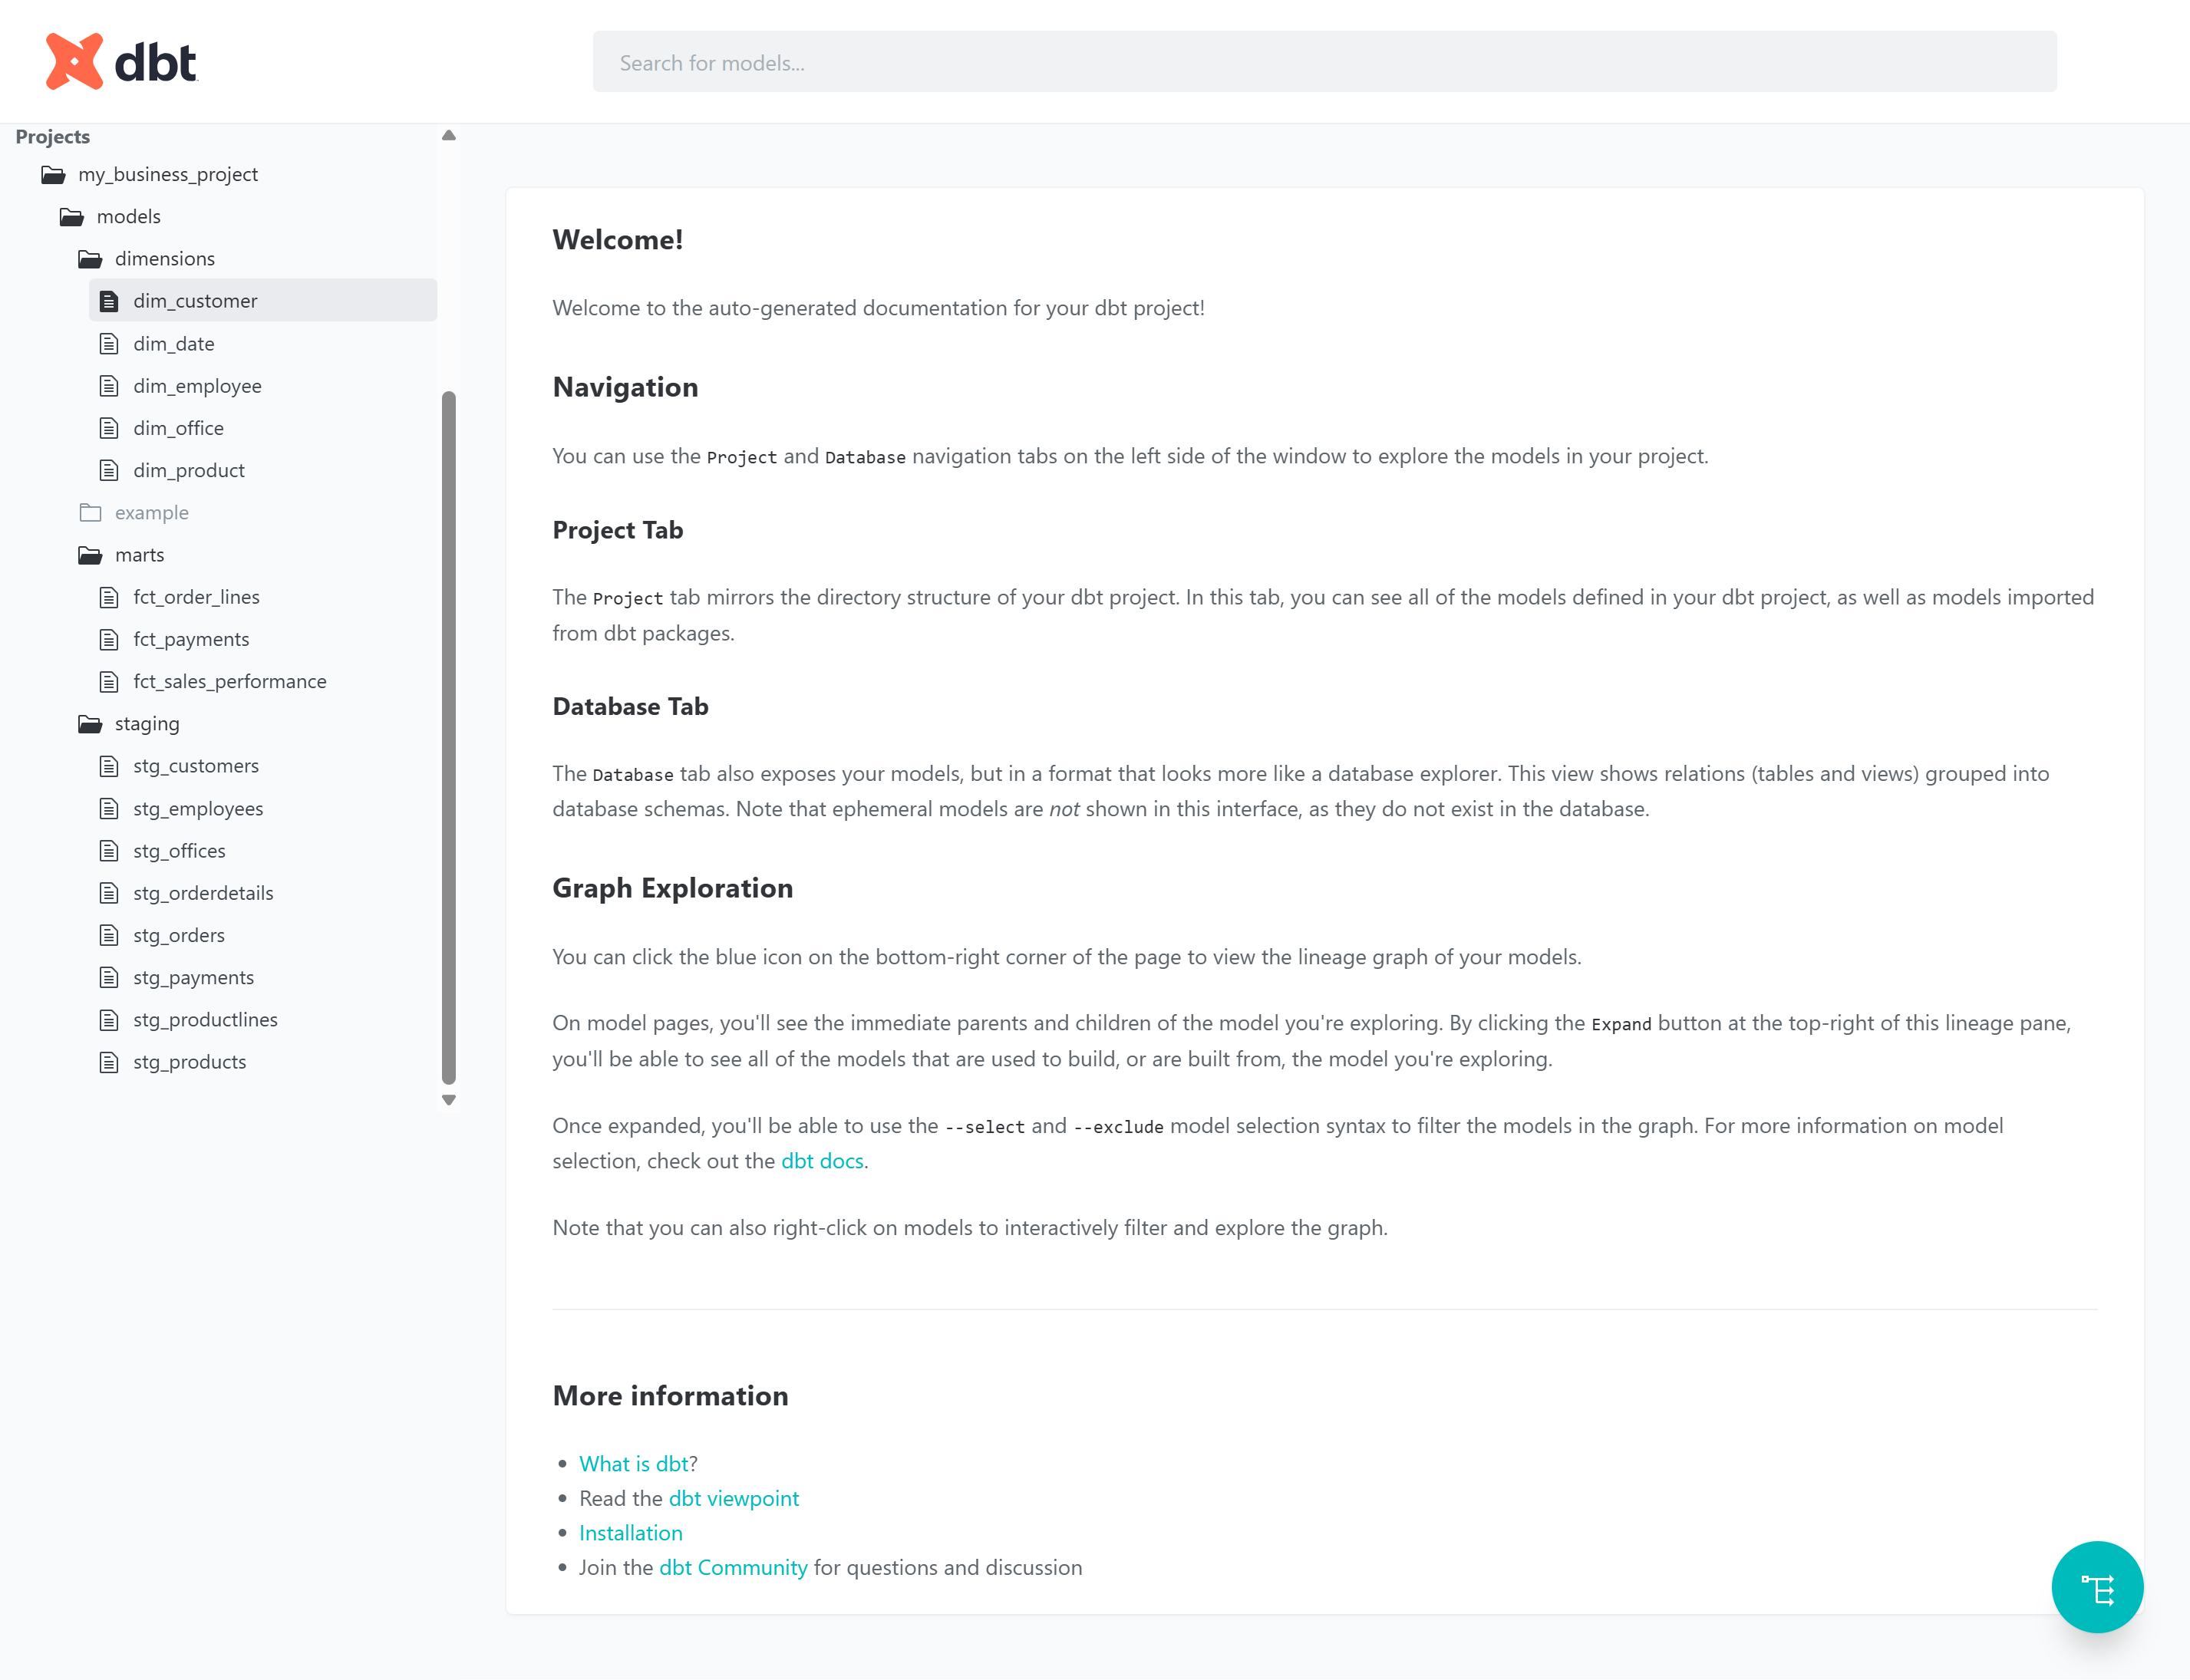
\includegraphics[width=0.95\textwidth]{figures/home-dbt.png}
    \caption{Dokumentasi yang diakses lewat localhost}
    \label{fig:home-dbt}
\end{figure}

\begin{figure}[H]
    \centering
    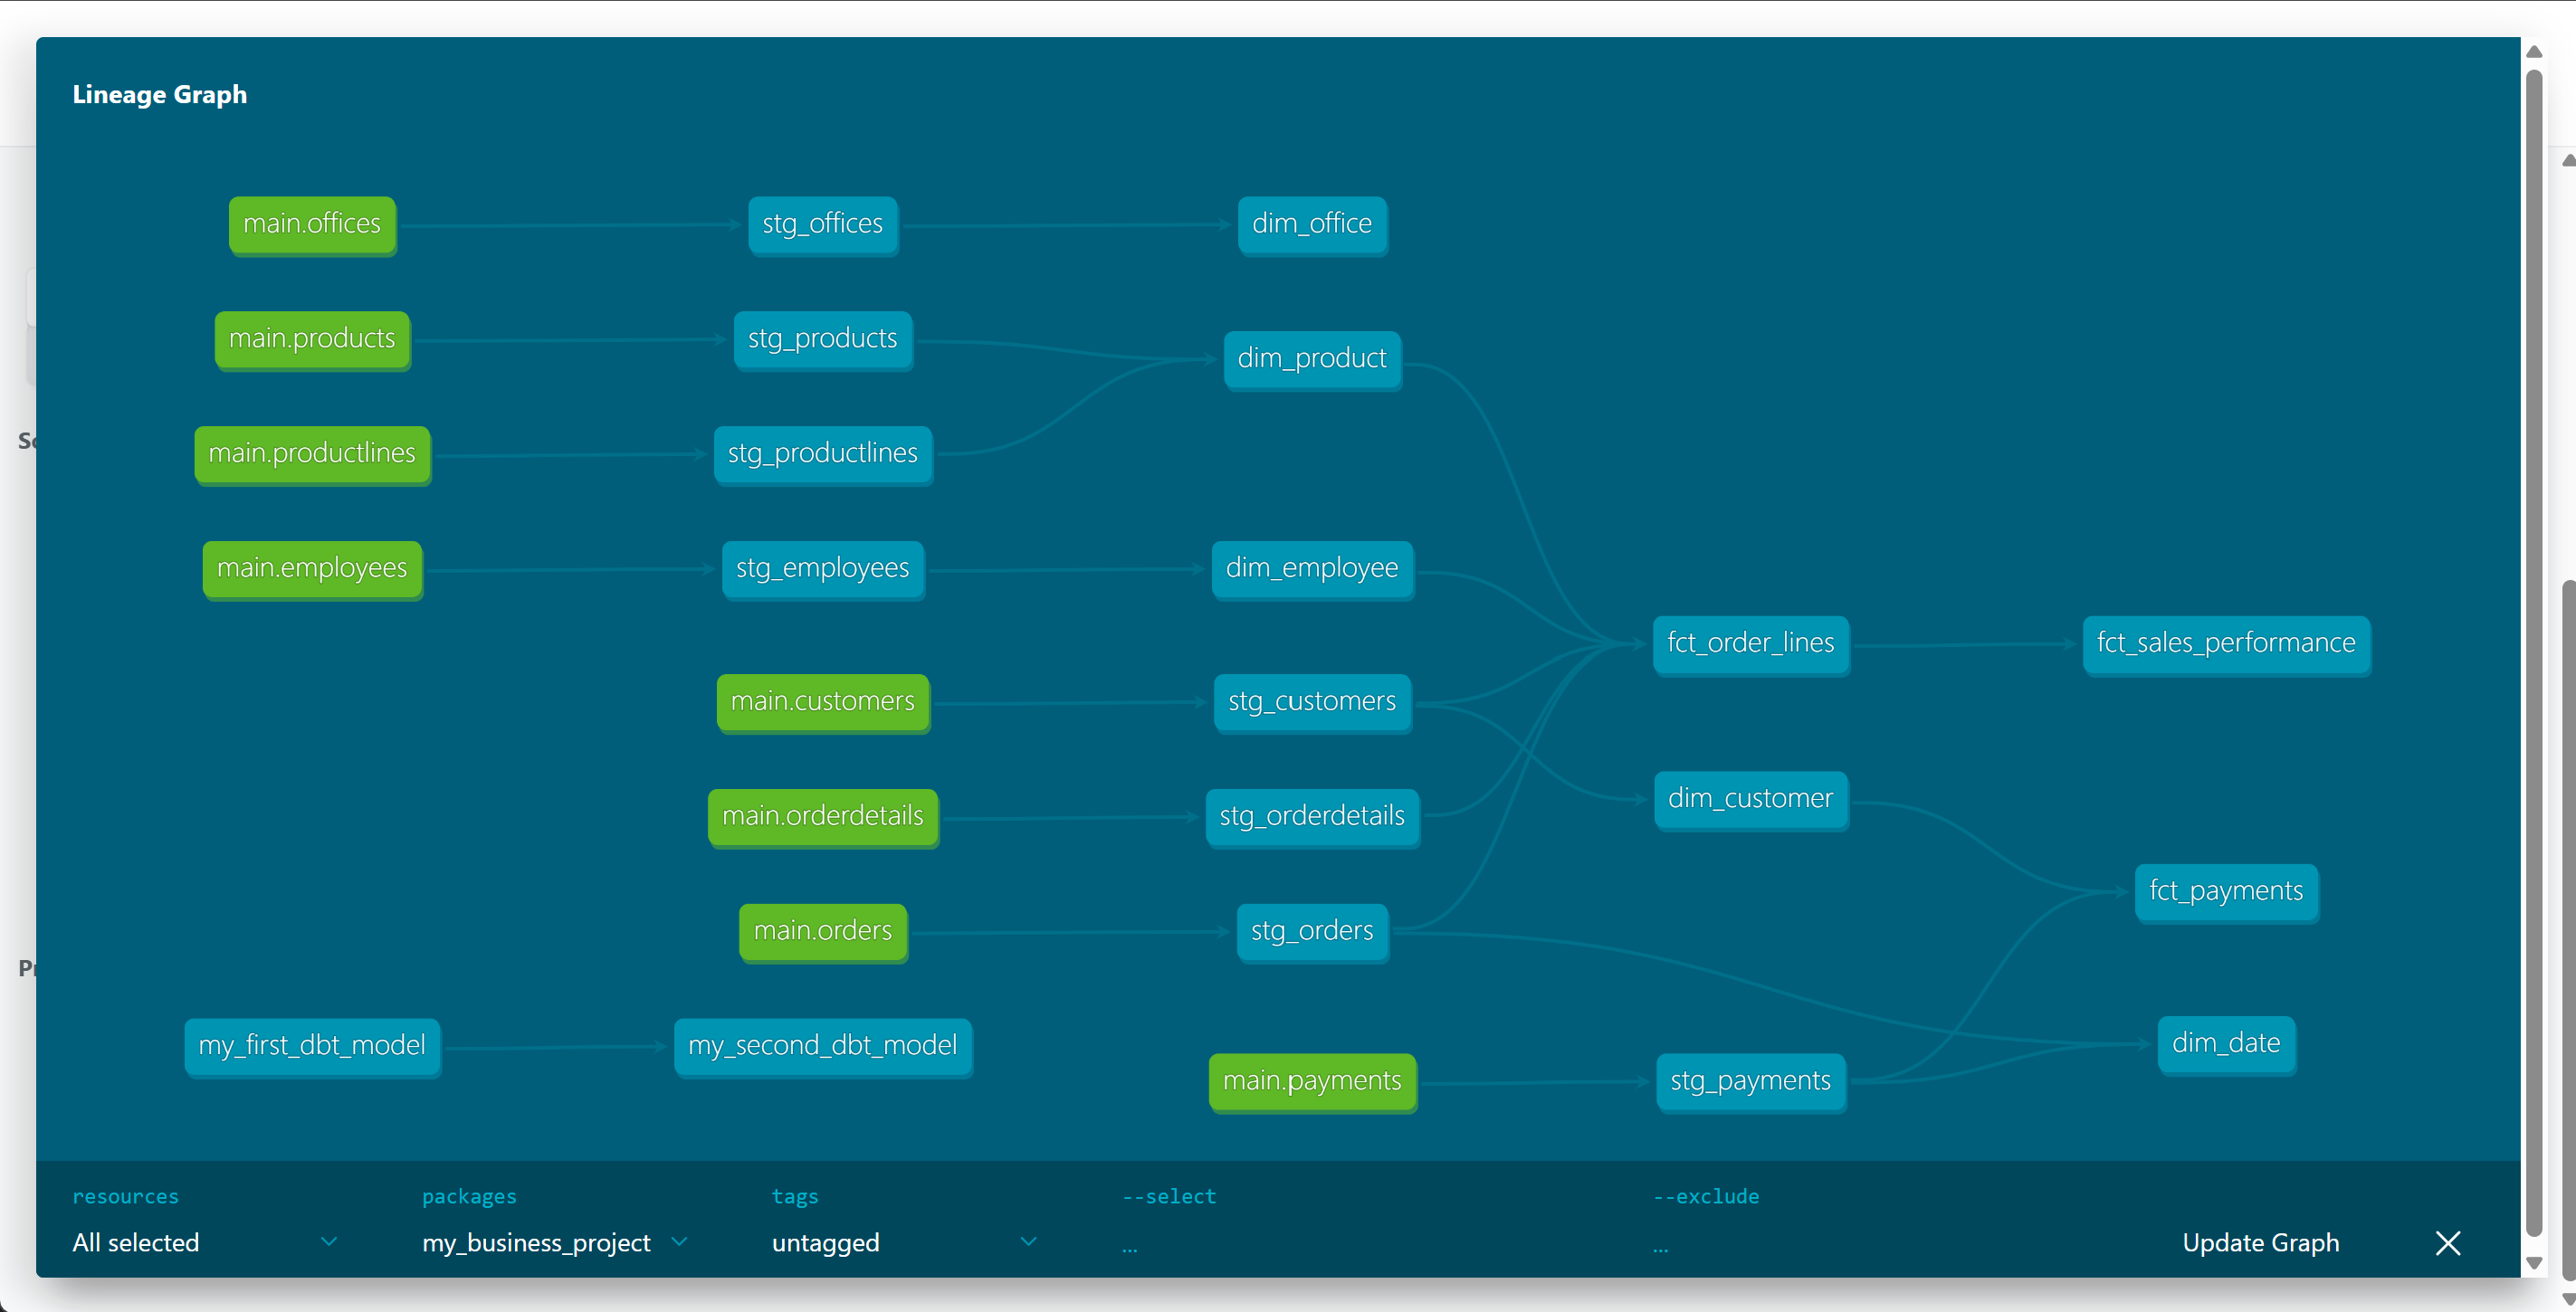
\includegraphics[width=0.95\textwidth]{figures/graph-dbt.png}
    \caption{Lineage Graph Interaktif yang menampilkan relasi antar lapisan staging, dimension dan fact}
    \label{fig:graph-dbt}
\end{figure}

\subsection{Analisis Lineage Graph (Silsilah Data)}

Berdasarkan grafik tersebut, alur data dibagi menjadi tiga tingkatan utama sesuai dengan prinsip \textit{Medallion Architecture}:

\begin{enumerate}
    \item \textbf{Source Layer (Main):} Titik awal data yang berasal dari database DuckDB (\texttt{main}). Terdapat empat tabel sumber utama yang diidentifikasi, yaitu \texttt{customers}, \texttt{orderdetails}, \texttt{orders}, dan \texttt{products}.
    \item \textbf{Staging Layer (Silver):} Data mentah ditransformasikan menjadi model \textit{staging} (\texttt{stg\_}). 
    \begin{itemize}
        \item \texttt{stg\_customers}, \texttt{stg\_orderdetails}, \texttt{stg\_orders}, dan \texttt{stg\_products} melakukan pembersihan awal (seperti penggantian nama kolom atau perubahan tipe data).
    \end{itemize}
    \item \textbf{Intermediate/Dimension Layer:} 
    \begin{itemize}
        \item \texttt{dim\_customer} mengambil referensi langsung dari \texttt{stg\_customers}.
        \item \texttt{dim\_product} mengambil referensi dari \texttt{stg\_products}.
    \end{itemize}
    \item \textbf{Mart/Fact Layer (Gold):} Puncak dari transformasi adalah tabel \texttt{fct\_order\_lines}. Tabel fakta ini memiliki ketergantungan (\textit{dependencies}) paling kompleks karena menggabungkan data dari \texttt{stg\_orderdetails}, \texttt{stg\_orders}, serta melakukan \textit{lookup} ke tabel dimensi \texttt{dim\_customer} dan \texttt{dim\_product}.
\end{enumerate}

\subsubsection{Fungsi dan Manfaat Lineage Graph}
\begin{itemize}
    \item \textbf{Data Traceability:} Memungkinkan pengembang untuk melacak asal-usul setiap kolom data. Jika ditemukan kesalahan pada \texttt{fct\_order\_lines}, pengembang dapat dengan mudah menelusuri ke belakang apakah kesalahan terjadi di level \textit{staging} atau pada data sumber.
    \item \textbf{Impact Analysis:} Sebelum melakukan perubahan pada tabel di level \textit{staging}, tim data dapat melihat model mana saja yang akan terdampak (misalnya, mengubah \texttt{stg\_products} akan berdampak pada \texttt{dim\_product} dan \texttt{fct\_order\_lines}).
    \item \textbf{Optimasi Kueri:} dbt menggunakan grafik ini untuk menentukan urutan eksekusi yang paling optimal
\end{itemize}
\clearpage
\subsection{Rincian Kontribusi Kelompok}
Seluruh tahapan dalam studi kasus ini dikerjakan secara kolaboratif dengan pembagian tanggung jawab yang mencakup penyusunan konten modul, penyiapan lingkungan teknis, hingga eksekusi transformasi data. Berikut adalah matriks kontribusi anggota kelompok yang merujuk pada struktur pembahasan dalam laporan ini:
\begin{table}[ht]
\centering
\caption{Rincian Kontribusi Anggota Kelompok Berdasarkan Struktur Laporan}
\label{tab:kontribusi-kelompok-detail}
\begin{tabular}{|c|l|p{8.5cm}|}
\hline
\textbf{No} & \textbf{Nama Anggota} & \textbf{Kontribusi Berdasarkan Struktur Bab} \\ \hline
1 & Engelbertus Rande & \textbf{Bab I (dbt Sebagai Tools Bantu):} Menyusun pengenalan dbt, konsep arsitektur, struktur model, serta dokumentasi standar \textit{Data Quality}. \\ \hline
2 & Gilbert Fandiliam Mooy & \textbf{Bab II (Penyiapan Lingkungan dbt):} Menyusun perbandingan dbt Core vs Cloud, dokumentasi instalasi \textit{package}, serta workflow inisialisasi proyek. \\ \hline
3 & Sinta Siti Nuriah & \textbf{Bab III (Studi Kasus - Fase Awal):} Menyusun skema DB/DW, konversi MySQL ke DuckDB, penyiapan \textit{Staging Layer}, serta implementasi \textit{Initial Code} dbt. \\ \hline
4 & Vicky Mahfudy & \textbf{Bab III (Studi Kasus - Fase Akhir):} Implementasi \textit{Dimensional Modeling} (Fakta \& Dimensi), optimasi \textit{Star Schema}, \textit{Data Exploration}, serta validasi kesesuaian antara modul dan teknis. \\ \hline
\end{tabular}
\end{table}